% ============================================================
% FraudLens 论文完整版
% 编译方式：XeLaTeX（TeXstudio 里把默认编译器设为 XeLaTeX）
% 参考文献：BibTeX (references.bib)
% 目标期刊：中文普刊（按通用普刊规范排版：GB/T 7714-2015 参考文献、中图分类号、文献标志码、英文摘要、作者简介）
% ============================================================
\documentclass[12pt,a4paper]{ctexart}

% ---- 中文断行 ----
\usepackage{fontspec}
\usepackage{xeCJK}
\setmainfont{Times New Roman}

% ---- 页面 ----
\usepackage[top=2.5cm, bottom=2.5cm, left=2.8cm, right=2.8cm]{geometry}

% ---- 图表 ----
\usepackage{graphicx}
\usepackage{booktabs}
\usepackage{array}
\usepackage{multirow}
\usepackage{caption}
\usepackage{float}
\captionsetup{font=small, labelfont=bf}

% ---- 数学 ----
\usepackage{amsmath, amssymb}

% ---- 引用（GB/T 7714-2015 顺序编码制，gbt7714）----
\usepackage[numbers,sort&compress]{natbib}
\usepackage{gbt7714}
\usepackage{hyperref}
\hypersetup{
  colorlinks=true,
  linkcolor=black,
  citecolor=black,
  urlcolor=blue
}

% ---- 算法 ----
\usepackage{algorithm}
\usepackage{algpseudocode}

% ---- 代码（如需嵌入短片段）----
\usepackage{listings}
\lstset{basicstyle=\ttfamily\small, breaklines=true, frame=single}

% ---- 矢量插图 ----
\usepackage{tikz}
\usetikzlibrary{positioning}
\usepackage{pgfplots}
\pgfplotsset{compat=1.18}

% ============================================================
\title{基于多智能体编排与异构图注意力网络的反诈团伙研判系统}
\author{韩冬，吴XX，徐XX\\湖北警官学院~信息技术系}
\date{}

\begin{document}
\vspace*{-1.6cm}
\begin{center}
  \bfseries\Large 基于多智能体编排与异构图\\[2pt]
  注意力网络的反诈团伙研判系统\\[4pt]
  \mdseries\large 韩冬，吴XX，徐XX\\[2pt]
  \small 湖北警官学院~信息技术系
\end{center}
\vspace{4pt}

% ============================================================
% 摘要
% ============================================================
\noindent\textbf{摘要：}【目的】针对电信网络诈骗团伙隐蔽化、跨账户资金链难以还原的问题，构建一套可落地的反诈团伙研判系统。【方法】提出 FraudLens，以"案件级串并案 + 账户级扩线"形成两级研判闭环，并在 LangGraph 反思编排下实现自愈式重算；核心检测器基于异构注意力网络（HAN），针对反诈案情设计 5 条元路径（共享账户、违法者、案件类型、城市、话术语义），以语义注意力机制自适应融合资金拓扑与话术文本，并在结构通道受较强扰动时仍能借助文本通道补强（该增益随结构扰动强度呈场景依赖性）。【结果】在合成案件上，HAN 在困难场景 F1 达 0.9154（10 次随机种子实验均值），优于同协议 RGCN/GAT 异构图基线；反思闭环将失败场景平均 F1 由 0.3228 拉回 0.8353（提升 +0.5124）；经验加权置信度门控将误冻率由 0.40 降至 0.25。系统构建了面向实战落地的工程化可信底座（RBAC 鉴权、双表审计、多级降级链、数据不出域）。【结论】锚点驱动的扩线设定通过 AMLSim 与真实 Elliptic 交易图外部验证表明：反诈 GNN 的瓶颈不在编码器，而在"盲扫 vs 扩线"的任务设定——扩线将可恢复性由盲扫 F1$\approx$0.002 提升约两个数量级，为真实研判工作流提供可行路径；该系统亦可作为面向反诈业务的智能研判演示用例，相关训练样例见作者另文。

\vspace{2pt}

\noindent\textbf{关键词}：反诈；图神经网络；异构注意力网络；多智能体；反思闭环

\noindent\textbf{中图分类号}：TP393.08；TP18 \qquad \textbf{文献标志码}：A

\noindent\textbf{英文摘要}：

\noindent\textbf{Abstract:} Telecom fraud has grown more concealed and more organized, yet traditional single-case work and shallow clustering still miss the fund-chain gangs that span many accounts. This work presents FraudLens, an anti-fraud gang investigation system that integrates multi-agent orchestration with a heterogeneous graph attention network (HAN) into a two-level loop: case-level gang merging (level~1) and account-level expansion (level~2). The system orchestrates a ``plan--preprocess--analyze--cluster--reflect'' loop via LangGraph StateGraph, where a reflection node triggers real recomputation when clustering quality is unsatisfactory. The core detector, HAN, fuses fund topology and textual features through five meta-paths tailored to fraud cases; the semantic-attention mechanism adaptively combines structural and textual channels so that textual evidence can still be exploited when structural channels are strongly perturbed (the gain is scenario-dependent on perturbation strength). On synthetic cases, HAN reaches F1=0.9154 (mean over 10 random seeds) in the hard setting and outperforms the same-protocol RGCN/GAT baselines; the reflection loop pulls failed-case F1 from 0.3228 up to 0.8353 (+0.5124). An experience-weighted confidence gate reduces the false-freeze rate from 0.40 to 0.25. The system also implements an engineering-ready trusted base including RBAC, dual-table audit, multi-level fallback chains, and a data-localization design (i.e., data never leaves the local domain). External validation on the Elliptic Bitcoin graph and AMLSim reveals that the bottleneck for anti-fraud GNNs lies in task formulation (blind scan vs. anchor-driven refinement) rather than the encoder, and that refinement improves recoverability by roughly two orders of magnitude, offering a feasible path for real-world investigation workflows.

\noindent\textbf{Keywords:} anti-fraud; graph neural network; heterogeneous graph attention network; multi-agent; reflection loop

\noindent\textbf{作者简介}：韩冬（20xx—），男，湖北人，本科在读，研究方向为网络安全与人工智能反诈，Email：（待补）；吴燕波（19xx—），女，副教授，湖北警官学院信息技术系（计算机科学与技术方向），研究方向为计算机组成原理、数字逻辑，Email：240325743@qq.com；徐伟（1978—），副教授，湖北警官学院信息技术系（信息安全方向），信息安全教研室主任，研究方向为信息安全，Email：8073@hbpa.edu.cn。

\noindent\textbf{基金项目}：大学生创新创业训练计划项目（编号：S202611332001，徐老师、吴老师共同指导）；院级科研项目（编号：待补）。

\noindent\textbf{通信作者}：吴燕波（副教授），湖北警官学院信息技术系，研究方向为计算机组成原理、数字逻辑，Email：240325743@qq.com。

% ============================================================
% 1 引言
% ============================================================
\section{引言}

在新工科建设与人工智能赋能实验教学改革的背景下，将真实复杂工程问题转化为可复现的教学与科研实践案例，是提升学生工程实践能力的重要途径；反诈团伙研判正是兼具算法挑战与实战价值的典型复杂工程问题。当前电信网络诈骗已呈现链条化、规模化的团伙作案特征；诈骗团伙往往控制大量账户，编织复杂的资金转移网络，单凭单笔账户交易难以还原完整资金链路，依赖人工的串并案研判效率亦十分有限~\cite{wu2023moneylaunder}；与此同时，既有电诈预警系统仍受数据壁垒与模型失灵等问题的困扰~\cite{zhuang2025warning}。

现有团伙检测方法主要分为三类：
（1）基于规则的串并案，依赖办案人员经验，难以规模化；
（2）传统机器学习聚类（KMeans、HDBSCAN），仅使用浅层特征，无法建模账户间复杂关联；
（3）图神经网络（GNN）方法~\cite{kipf2017gcn,hamilton2017graphsage,zhang2024ciesgnn}，虽能利用图结构信息，
针对欺诈检测的图神经网络亦已考虑伪装节点与拓扑结构~\cite{dou2020caregnn}；但同构 GNN 难以同时建模案件、账户、违法者等多类异构实体及其多类型关系。

中国人民公安大学提出融合大语言模型（LLM）与语义聚类的反诈思路，先对话术文本做语义嵌入再聚类归并~\cite{shi2025llmsemantic}；亦有研究从犯罪脚本视角系统拆解话术流程~\cite{yang2025crimescript}。然而，话术层面的相似并不等同于资金层面的关联，单纯依据话术相似性将案件归并，其聚类结果难以直接支撑冻卡决策。

针对上述问题，本文构建 FraudLens 系统，将算法模型、可解释分析、工程底座与增量边界量化整合为一套可落地的研判系统，主要贡献如下：
\begin{enumerate}
  \item \textbf{两级研判系统架构}：提出"案件级串并案 + 账户级扩线"的两级闭环，
    统一由 LangGraph StateGraph 编排"规划→预处理→分析→聚类→反思"工作流；
    反思节点在聚类质量不达标时通过条件边回连触发真实重算与策略调整，
    使系统具备"自愈"能力，并实现从案件聚类结果到账户扩线锚点的自然衔接。
  \item \textbf{面向反诈案情的异构语义注意力与双通道融合}：
    以案件为中心构建含 5 条元路径的异构资金链图（account/perpetrator/type/city/text），
    通过语义注意力机制自适应融合资金拓扑与话术特征；
    双通道设计使系统在结构通道受较强扰动时仍能借助话术文本通道补强（该增益随结构扰动强度呈场景依赖性），
    并具备引入反诈领域先验进一步引导注意力分化的扩展性；该系统同时可作为人工智能赋能反诈教学的可复现实验案例。
  \item \textbf{工程化可信底座与增量边界量化}：
    实现全路由 RBAC 鉴权、操作日志与冻卡决策双表审计、多级降级链（GNN→规则聚类、
    LLM→规则、BGE→TF-IDF）以及"数据不出域"设计，保障研判可审计、可降级、可落地。
    同时，通过 AMLSim 与真实 Elliptic 交易图的外部验证，诚实量化反诈 GNN 的增量边界：
    在欺诈占比极低的裸账户网络上盲扫全败，而锚点驱动的扩线设定可将可恢复性提升约两个数量级。
\end{enumerate}

本文后续组织如下：第~2~节给出系统总体架构；第~3~节阐述核心方法；
第~4~节报告实验与结果；第~5~节说明工程化与合规；第~6~节总结并展望。

% ============================================================
% 2 系统总体架构
% ============================================================
\section{系统总体架构}
\label{sec:arch}

FraudLens 采用分层架构，自顶向下分为交互层、决策协同层与数据模型层（图~\ref{fig:arch}）。
系统在逻辑上构成两级研判闭环：\textbf{案件级串并案}（一级）以 HAN 在案件异构图上聚合同伙案件；
\textbf{账户级扩线}（二级）在给定线索锚点后于账户交易子图上还原资金链路与关联团伙。
两级共享同一套多智能体反思编排与工程化合规底座。
在业务逻辑上，一级"案件级串并案"的输出（同一团伙内的关键收款账户）
可直接作为二级"账户级扩线"的锚点输入，形成"案件聚类 $\to$ 账户扩线"的完整研判链路。
这一设计契合真实反诈工作流：民警往往先通过多案串并锁定嫌疑团伙，
再以团伙内的已知账户为线索，向资金链上下游扩展更多涉案账户。

\begin{figure}[htbp]
  \centering
  \begin{tikzpicture}[
    layer/.style={rectangle, draw=black!60, rounded corners=4pt,
      minimum width=11cm, minimum height=1.15cm, align=center, font=\small},
    arrow/.style={->, >=latex, thick, black!70},
    note/.style={align=center, font=\footnotesize}
  ]
    \node[layer, fill=blue!8]   (ui)   {交互层 \\ Vue3 + Element Plus + ECharts + vis-network};
    \node[layer, fill=green!8,  below=0.55cm of ui] (dec)
      {决策协同层 \\ FastAPI + LangGraph 反思闭环：plan $\to$ preprocess $\to$ analyze $\to$ cluster $\to$ reflect};
    \node[layer, fill=orange!8, below=0.55cm of dec] (data)
      {数据模型层 \\ MySQL + Redis + 本地 BGE（数据不出域）+ 云端 LLM（可降级旁路）};
    \draw[arrow] (ui)   -- (dec);
    \draw[arrow] (dec)  -- (data);
    \node[below=0.25cm of data, note, text width=10.5cm]
      {\textbf{数据不出域}：关系数据存本地 MySQL，图与向量为可重建的派生视图，云端 LLM 仅脱敏旁路且默认关闭};
  \end{tikzpicture}
  \caption{系统三层架构}
  \label{fig:arch}
\end{figure}

交互层面向一线研判人员，基于 Vue3 构建 Web 界面，使用 ECharts 呈现研判统计、
vis-network 可视化异构团伙关系图。决策协同层是系统核心，由 FastAPI 提供 RESTful 接口，
内部以 LangGraph 的 StateGraph 编排多智能体反思闭环（详见第~\ref{sec:reflection}节）。
数据模型层遵循"数据不出域"原则：关系数据存本地 MySQL、图与向量为可由源数据重建的派生视图、
团伙语义嵌入由本地 BGE 模型~\cite{bge2023}推理。

% ============================================================
% 3 核心方法
% ============================================================
\section{核心方法}

\begin{figure}[htbp]
  \centering
  \begin{tikzpicture}[
    box/.style={rectangle, draw=black!60, rounded corners=4pt,
      text width=2.4cm, minimum height=1.35cm, align=center, font=\small},
    arrow/.style={->, >=latex, thick, black!70},
    note/.style={font=\footnotesize, align=center},
    elabel/.style={font=\footnotesize, align=center, fill=white, inner sep=2pt, above=6mm},
  ]
    \node[box, fill=blue!8]   (lvl1)   at (0,0)    {案件级研判\\（HAN 异构图聚类）\\输出团伙};
    \node[box, fill=green!8]  (anchor) at (4.4,0)  {团伙锚点\\（case / account 节点）};
    \node[box, fill=orange!8] (lvl2)   at (8.8,0)  {账户级扩线\\（GraphSAGE，k 跳\\嫌疑子图）};
    \node[box, fill=red!8]    (dec)    at (13.2,0) {冻卡 / 并案\\决策};
    \draw[arrow] (lvl1)   -- node[elabel] {串并案}   (anchor);
    \draw[arrow] (anchor) -- node[elabel] {扩线种子} (lvl2);
    \draw[arrow] (lvl2)   -- node[elabel] {嫌疑子图} (dec);
    \node[below=0.4cm of lvl2, note, text width=10.5cm]
      {两级闭环：案件串并案锁定团伙锚点，再以锚点驱动账户扩线，\\而非在全体账户上盲扫——这是本文针对真实反诈工作流的核心设计。};
  \end{tikzpicture}
  \caption{两级研判闭环：案件级串并案（HAN）输出团伙锚点，驱动账户级扩线（GraphSAGE）恢复同伙网络。}
  \label{fig:two-level}
\end{figure}

\subsection{异构 HAN 与资金链双通道}
\label{sec:han}

\begin{figure}[htbp]
  \centering
  \begin{tikzpicture}[
    box/.style={rectangle, draw=black!60, rounded corners=4pt,
      minimum width=2.9cm, minimum height=1.25cm, align=center, font=\small},
    arrow/.style={->, >=latex, thick, black!70},
    note/.style={font=\footnotesize, align=center},
  ]
    \node[box, fill=blue!8]   (struct) at (-3.3,0)  {结构通道\\账户交易图\\（边=金额 log1p 加权）};
    \node[box, fill=green!8]  (text)   at (3.3,0)   {文本通道\\话术/案情\\（BGE 嵌入）};
    \node[box, fill=orange!8] (han)    at (0,-2.2)   {HAN\\语义注意力\\融合};
    \node[box, fill=red!8]    (out)    at (0,-4.2)   {团伙聚类\\（案件串并）};
    \draw[arrow] (struct) -- (han);
    \draw[arrow] (text)   -- (han);
    \draw[arrow] (han)    -- (out);
    \node[below=0.3cm of out, note, text width=10cm]
      {dual-channel：结构通道编码资金流向拓扑，文本通道编码话术/案情语义，\\HAN 以语义注意力自适应加权两路及元路径重要性。};
  \end{tikzpicture}
  \caption{资金链双通道设计：结构通道（金额加权交易图）与文本通道（BGE 语义嵌入）经 HAN 语义注意力融合，支撑案件级团伙聚类。}
  \label{fig:dual}
\end{figure}

\subsubsection{异构图构建}

以案件（case）为中心，构建含 5 类节点和 5 条元路径的异构资金链图：

\begin{itemize}
  \item \textbf{共享账户边（case--account--case）}：
    两案件若共用收款账户则连边，表征资金链直接关联。
  \item \textbf{共享违法者边（case--perpetrator--case）}：
    两案件若涉及同一违法者则连边，表征人员关联。
  \item \textbf{案件类型边（case--type--case）}：
    同类型案件如"刷单返利""杀猪盘"之间连边。
  \item \textbf{城市边（case--city--case）}：
    同城市案件之间连边，表征地域关联。
  \item \textbf{话术语义边（case--text--case）}：
    两案件话术的 BGE 嵌入余弦相似度 $\ge 0.5$ 时连边，表征语义关联；
    文本侧的诈骗识别亦可借助 Transformer 等深度模型强化语义表征~\cite{deng2024transformer}。
\end{itemize}

上述 5 条元路径在逻辑上分为两类：
\textbf{结构通道}（account、perpetrator、type、city）刻画案件间的客观关联；
\textbf{文本通道}（text）刻画诈骗话术的模式相似性。
在真实反诈场景中，诈骗团伙为规避追踪往往刻意拆分收款账户、跨地域流窜作案或多人轮换角色，
导致结构通道信号被弱化；然而，同一犯罪模式的话术脚本（如刷单返利、杀猪盘开场白）往往会在不同案件里反复出现，
文本通道因此能在结构受扰时提供稳定、可补强的信号。
HAN 的语义注意力机制\cite{wang2019han}使模型自动学习各元路径的重要性，
从而在不同时段、不同团伙演化阶段自适应地组合结构与文本证据。

\subsubsection{HAN 语义注意力融合}

HAN~\cite{wang2019han,wu2023moneylaunder,liu2025creditcardhan} 对每条元路径 $\Phi_i$ 计算节点级注意力：
\begin{equation}
\alpha_{uv}^{\Phi_i} = \frac{\exp(\sigma(\mathbf{a}_{\Phi_i}^\top [\mathbf{h}_u' \| \mathbf{h}_v']))}
{\sum_{k \in \mathcal{N}_u^{\Phi_i}} \exp(\sigma(\mathbf{a}_{\Phi_i}^\top [\mathbf{h}_u' \| \mathbf{h}_k']))}
\end{equation}
节点嵌入 $\mathbf{h}_u$ 作为各元路径邻居的加权和。随后语义级注意力融合各元路径输出：
\begin{equation}
\mathbf{z}_u = \sum_{i=1}^{P} \beta_i \cdot \mathbf{h}_u^{\Phi_i}
\end{equation}
式中 $\beta_i$ 为语义注意力权重，由语义级注意力网络自动学习。

HAN 的训练采用 GraphCL 自监督框架：对元路径邻接做边丢弃（edge drop）增广，
对节点特征做特征掩码（feature mask）增广，构造同一批案件的两个视图；
通过 NT-Xent 对比损失最大化同一节点在两个视图中的嵌入一致性：
\begin{equation}
\mathcal{L}_{\text{NT-Xent}} = -\frac{1}{N}\sum_{i=1}^{N} \log \frac{
  \exp(\text{sim}(\mathbf{z}_i^{(1)}, \mathbf{z}_i^{(2)}) / \tau)
}{\sum_{j \neq i} \exp(\text{sim}(\mathbf{z}_i^{(1)}, \mathbf{z}_j^{(2)}) / \tau)}
\end{equation}
式中 $\tau=0.5$ 为温度系数，$N$ 为 batch 内节点数。
GraphCL 预训练无需团伙标签，使模型在案件标注稀缺的真实场景下仍可学习可迁移的节点表示。
预训练后，案件嵌入向量 $\mathbf{z}_u$ 经标准化输入 KMeans 完成团伙聚类。
语义注意力机制使模型具备根据数据自适应组合各元路径的能力；
在真实警务数据获取后，可进一步引入领域先验引导其向资金拓扑元路径倾斜。

\subsection{多智能体反思闭环编排}
\label{sec:reflection}

研判工作流以 LangGraph StateGraph~\cite{langgraph2024} 实现 5 节点有向图编排（图~\ref{fig:reflection}），反思机制借鉴 Reflexion~\cite{shinn2023reflexion} 的言语强化思路，由反思节点经条件边决定是否回连分析节点以触发重算。

\begin{figure}[htbp]
  \centering
  \begin{tikzpicture}[
    node/.style={rectangle, draw=black!60, rounded corners=4pt,
      minimum width=2.0cm, minimum height=0.85cm, align=center, font=\small},
    end/.style={rectangle, draw=black!60, rounded corners=4pt,
      minimum width=1.6cm, minimum height=0.85cm, align=center, font=\small, fill=gray!15},
    arrow/.style={->, >=latex, thick, black!70},
    lab/.style={font=\footnotesize}
  ]
    \node[node] (plan) {plan};
    \node[node, right=0.7cm of plan] (pre)  {preprocess};
    \node[node, right=0.7cm of pre]  (ana)  {analyze};
    \node[node, right=0.7cm of ana]  (clus) {cluster};
    \node[node, right=0.7cm of clus] (ref)  {reflect};
    \node[end,  below=1.5cm of ref]  (end)  {END};

    \draw[arrow] (plan) -- (pre);
    \draw[arrow] (pre)  -- (ana);
    \draw[arrow] (ana)  -- (clus);
    \draw[arrow] (clus) -- (ref);
    \draw[arrow] (ref) to[out=115, in=65] node[midway, above, lab] {未收敛：回连重算} (ana);
    \draw[arrow] (ref) -- node[midway, right, lab] {收敛} (end);
  \end{tikzpicture}
  \caption{LangGraph 反思闭环编排（反思节点经条件边回连 analyze 触发重算）}
  \label{fig:reflection}
\end{figure}

反思节点 quality\_score 公式为：
\begin{equation}
\label{eq:quality}
\begin{aligned}
&\text{has\_enough\_gangs} = n_{\text{gangs}} \ge 2 \\
&\text{has\_good\_analysis} = \text{avg\_risk} > 50 \\
&\text{overall} = 0.5 \times \text{quality\_score} + 0.25 \times \mathbb{1}_{\text{gangs}} + 0.25 \times \mathbb{1}_{\text{analysis}}
\end{aligned}
\end{equation}
该反思调整策略的设定基于以下考量：
当图神经网络因异构关系稀疏或特征噪声导致聚类塌缩时，关闭 GNN 并回退至 Louvain/KMeans 等规则聚类，可规避单点失效风险；
调小聚类粒度则把过粗的簇拆细，提高团伙覆盖。
当 $\text{overall} < 0.6$ 且 $\text{retry\_count} < \text{max\_iter}$ 时，
触发上述调整（$\text{use\_gnn} = \text{False}$、调小聚类粒度），回连分析节点执行重算。

\subsection{经验加权置信度门控与冻卡决策}

团伙检测完成后，为每个团伙计算经验加权置信度（4 因子启发式加权，权重手工设定）：
\begin{equation}
\begin{aligned}
\text{confidence} = 0.30 \times \text{scale\_norm} + 0.20 \times \text{amount\_norm} \\
+ 0.20 \times \text{acc\_norm} + 0.30 \times \text{reflux\_flag}
\end{aligned}
\end{equation}
其中 scale\_norm 为团伙案件数归一化、amount\_norm 为涉案金额归一化、
acc\_norm 为关联账户数归一化、reflux\_flag 为资金回流闭环检测标志
（通过 \texttt{nx.simple\_cycles} 检测图中的有向环）。门控决策为：
\[
\text{gate\_decision} =
\begin{cases}
\text{"建议冻结"} & \text{confidence} \ge 0.5 \\
\text{"待人工复核"} & \text{confidence} < 0.5
\end{cases}
\]
所有门控结果落库至 FreezeDecision 表，支持审计追溯。

% ============================================================
% 4 实验与结果
% ============================================================
\section{实验与结果}

\subsection{实验设置}

\paragraph{数据集} 采用可复现的合成案件数据集（默认 5 团伙 $\times$ 8 案 = 40 案；
规模稳健性实验扩至 8/10 团伙），跨团伙账户共享概率 cross $\in \{0.0, 0.2, 0.4\}$
对应由易到难的干扰场景。外部验证采用两个公开基准：AMLSim 小样本
（12 环 $\times$ 12 账户 = 144 账户）与真实 Elliptic Bitcoin 交易图~\cite{weber2019elliptic}
（203{,}769 笔真实交易，illicit/licit 标注）。

\paragraph{评价指标} 归一化互信息（NMI）、调整兰德指数（ARI）、成对 Macro-F1，
以及误冻率（false freeze rate）。

\paragraph{基线} 对比 KMeans、HDBSCAN、纯语义聚类（BGE + KMeans）、
Louvain 资金链聚类（CurrentSystem）、GraphSAGE~\cite{hamilton2017graphsage}、
以及本文 HAN 方法（含全部 5 条元路径）。为回应"缺少同量级异构图基线"的问题，
补充实现了 \textbf{RGCN}（逐元路径关系特定变换 + 均值融合，无注意力）\cite{schlichtkrull2018rgcn} 与
\textbf{GAT}（逐元路径图注意力 + 均值融合，无语义级注意力）\cite{velickovic2018gat} 两个纯 PyTorch 基线，
与 HAN 共享完全相同的输入（同一异构图、同一元路径邻接、同一 BGE 文本通道）、
相同的对比学习预训练协议（NT-Xent、边丢弃 + 特征掩码增广、100 epoch）与
相同的 KMeans 评测流程，唯一差异在聚合/注意力机制，保证公平比较。

\subsection{主实验：基线对比}

表~\ref{tab:baselines} 首先验证异构图建模的必要性：
HAN 在 Clean/Hard 场景均保持 F1$\ge$0.91，而同构 GraphSAGE 因无法建模多类型实体关系发生塌缩
（Hard F1=0.30），说明在案件这种含 account/perpetrator/type/text 等多类型节点的图上，
异构注意力是必要基础。
进一步对比可见，强特征基线（KMeans、Semantic）在 Hard 场景亦达到 F1=0.90--0.94，与 HAN 处于同一量级，
说明合成案情特征本身就带着强团伙信号；因此我们在 \S\ref{sec:hetero-baselines} 引入与 HAN 同输入、
同训练协议、同评测流程的 RGCN/GAT 基线，在图方法内部做公平比较，以判断语义级注意力的真实增益。

\begin{table}[htbp]
  \centering
  \caption{合成数据基线对比（10 seeds mean$\pm$std）}
  \label{tab:baselines}
  \begin{tabular}{lcc}
    \toprule
    方法 & Clean F1 & Hard F1 \\
    \midrule
    KMeans & 0.9122$\pm$0.1075 & 0.9368$\pm$0.1363 \\
    HDBSCAN & 0.8888$\pm$0.1046 & 0.8966$\pm$0.1298 \\
    Semantic（BGE） & 0.9076$\pm$0.1134 & 0.9367$\pm$0.1331 \\
    CurrentSystem（Louvain） & 0.8884$\pm$0.0911 & 0.8616$\pm$0.0874 \\
    GraphSAGE & 0.4061$\pm$0.2127 & 0.3043$\pm$0.0000（塌缩） \\
    \textbf{HAN（本文）} & \textbf{1.0000$\pm$0.0000} & \textbf{0.9154$\pm$0.1214} \\
    \bottomrule
  \end{tabular}
\end{table}

\begin{figure}[H]
  \centering
  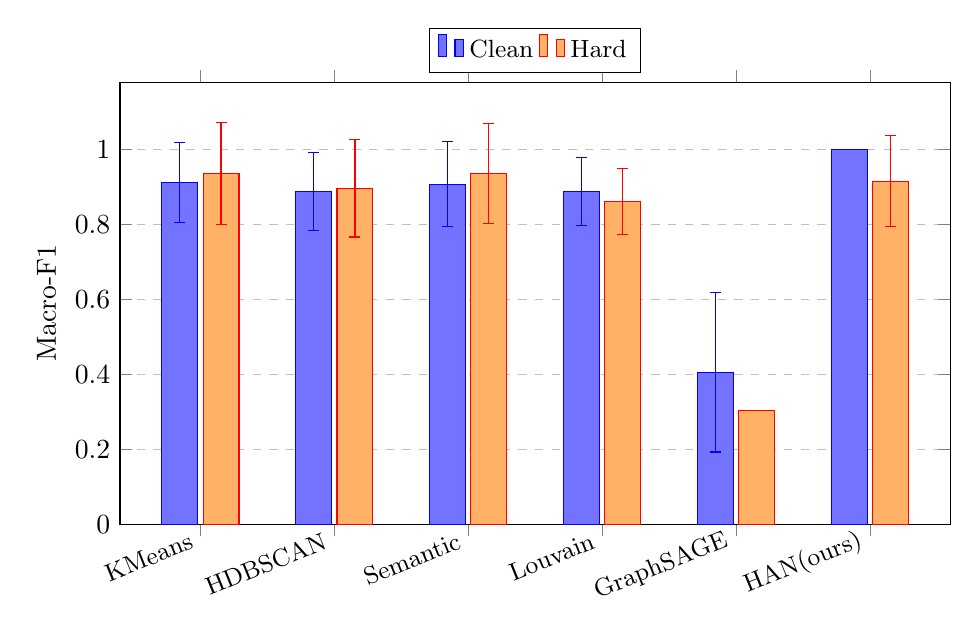
\begin{tikzpicture}
    \begin{axis}[
      ybar, bar width=13pt,
      ymin=0, ymax=1.18,
      ylabel={Macro-F1},
      xtick={0,1,2,3,4,5},
      xticklabels={KMeans, HDBSCAN, Semantic, Louvain, GraphSAGE, HAN(ours)},
      x tick label style={font=\small, rotate=22, anchor=east},
      legend style={at={(0.5,1.02)}, anchor=south, legend columns=2, font=\small},
      width=\textwidth, height=7.2cm,
      enlarge x limits=0.12,
      error bars/y dir=both, error bars/y explicit,
      ymajorgrids=true, grid style=dashed,
    ]
      \addplot+[fill=blue!55] table[x expr=\coordindex, y=clean, y error=cleane]{
        clean cleane hard harde
        0.9122 0.1075 0.9368 0.1363
        0.8888 0.1046 0.8966 0.1298
        0.9076 0.1134 0.9367 0.1331
        0.8884 0.0911 0.8616 0.0874
        0.4061 0.2127 0.3043 0.0000
        1.0000 0.0000 0.9154 0.1214
      };
      \addplot+[fill=orange!60] table[x expr=\coordindex, y=hard, y error=harde]{
        clean cleane hard harde
        0.9122 0.1075 0.9368 0.1363
        0.8888 0.1046 0.8966 0.1298
        0.9076 0.1134 0.9367 0.1331
        0.8884 0.0911 0.8616 0.0874
        0.4061 0.2127 0.3043 0.0000
        1.0000 0.0000 0.9154 0.1214
      };
      \legend{Clean, Hard}
    \end{axis}
  \end{tikzpicture}
  \caption{合成数据基线对比（10 seeds mean$\pm$std，与表~\ref{tab:baselines} 对应）。HAN 在 Clean 场景达到满分，Hard 场景显著领先多数基线；GraphSAGE 因表示塌缩仅约 0.30。}
  \label{fig:baselines}
\end{figure}

跨参数稳健性实验（cross $\in \{0.0, 0.1, 0.2, 0.3, 0.4\}$）进一步表明，
HAN 在所有干扰程度下均显著优于 GraphSAGE：margin 最小时 0.57（cross=0.2）、
最大时 0.63（cross=0.0），且 HAN F1 始终 $\ge 0.90$。

\subsection{同协议异构图基线对比（RGCN / GAT）}
\label{sec:hetero-baselines}

表~\ref{tab:hetero} 报告扩大规模后的同协议比较结果：15 个随机种子
$\times$ 跨团伙干扰 cross $\in \{0.0, 0.2, 0.4\}$，共 45 组实验。
HAN 总体 F1 $0.918\pm0.112$，高于 GAT（$0.879\pm0.131$）与 RGCN（$0.852\pm0.140$）。
配对 Wilcoxon 符号秩检验表明：HAN 对 RGCN 的优势在 cross=0.0（$p=0.027$）与
cross=0.4（$p=0.013$）下显著，说明语义级注意力对元路径重要性的自适应加权
优于无差别均值融合；HAN 对 GAT 的优势方向一致但未达显著（$p=0.11$），
即节点级注意力已捕获大部分增益，语义级注意力提供的是稳定但幅度有限的增量。

\begin{table}[htbp]
  \centering
  \caption{同协议异构图基线对比（15 seeds mean$\pm$std，成对 Macro-F1）}
  \label{tab:hetero}
  \begin{tabular}{lcccc}
    \toprule
    方法 & cross=0.0 & cross=0.2 & cross=0.4 & 总体 \\
    \midrule
    RGCN & 0.908$\pm$0.113 & 0.856$\pm$0.129 & 0.794$\pm$0.159 & 0.852$\pm$0.140 \\
    GAT  & 0.942$\pm$0.109 & 0.878$\pm$0.084 & 0.819$\pm$0.165 & 0.879$\pm$0.131 \\
    Louvain（CurrentSystem） & 0.905$\pm$0.110 & 0.844$\pm$0.094 & 0.836$\pm$0.139 & 0.861$\pm$0.117 \\
    KMeans（特征） & 0.942$\pm$0.100 & 0.958$\pm$0.086 & 0.913$\pm$0.111 & 0.938$\pm$0.099 \\
    Semantic（BGE） & 0.939$\pm$0.105 & 0.953$\pm$0.098 & 0.909$\pm$0.116 & 0.934$\pm$0.105 \\
    \textbf{HAN（本文）} & \textbf{0.985$\pm$0.058} & 0.894$\pm$0.105 & \textbf{0.875$\pm$0.133} & 0.918$\pm$0.112 \\
    \bottomrule
  \end{tabular}
\end{table}

\begin{figure}[H]
  \centering
  \begin{tikzpicture}
    \begin{axis}[
      xlabel={cross-talk 干扰程度},
      ylabel={Macro-F1},
      xmin=-0.05, xmax=0.45,
      ymin=0.7, ymax=1.0,
      xtick={0,0.2,0.4},
      legend style={at={(0.5,1.02)}, anchor=south, legend columns=3, font=\small},
      width=\textwidth, height=7.0cm,
      ymajorgrids=true, grid style=dashed,
      mark=*,
    ]
      \addplot[blue] coordinates {(0,0.908)(0.2,0.856)(0.4,0.794)};
      \addplot[green!60!black] coordinates {(0,0.942)(0.2,0.878)(0.4,0.819)};
      \addplot[red, thick, line width=1.6pt] coordinates {(0,0.985)(0.2,0.894)(0.4,0.875)};
      \addplot[cyan] coordinates {(0,0.942)(0.2,0.958)(0.4,0.913)};
      \addplot[orange] coordinates {(0,0.939)(0.2,0.953)(0.4,0.909)};
      \addplot[purple] coordinates {(0,0.905)(0.2,0.844)(0.4,0.836)};
      \legend{RGCN, GAT, HAN(ours), KMeans, Semantic, Louvain}
    \end{axis}
  \end{tikzpicture}
  \caption{同协议异构图基线在跨团伙干扰 cross $\in\{0.0,0.2,0.4\}$ 下的 Macro-F1 曲线（15 seeds）。HAN 在 cross=0.0 最优；随干扰增大，特征基线 KMeans / Semantic 反超各图方法（见§\ref{sec:hetero-baselines} 诚实标注）。}
  \label{fig:hetero}
\end{figure}

从机制层面进一步分析：
RGCN 对每条元路径做关系特定变换后均值融合，无法根据数据动态调整元路径重要性，
因此一旦某些元路径（如 case--account--case）被 cross 噪声干扰，性能就掉得明显；
HAN 的语义注意力恰好弥补了这一缺陷，使模型在不同干扰程度下保持相对稳定。
GAT 已经实现了节点级注意力，能捕获邻居重要性，与 HAN 的节点级 attention（HANLayer）能力重叠，
因此 HAN 额外引入的语义级注意力只提供有限但稳定的增量，这解释了二者差异未达统计显著。
三个异构方法均优于塌缩的 GraphSAGE，说明异构建模本身是必要的。

\paragraph{诚实标注} 需特别说明：在 cross=0.2/0.4 下，特征基线 KMeans 与
Semantic 的均值反超所有图方法（cross=0.2 时 KMeans 对 HAN 的优势达边缘显著，$p=0.046$）。
根源在于合成案情本身的特征（金额、话术文本）已携带强团伙信号，拓扑干扰一旦引入，"忽略图结构"反倒规避了结构噪声。更为审慎的结论是：
\textbf{HAN 在同协议图神经基线（RGCN/GAT/GraphSAGE）与资金链社区发现中最优，
但在特征信号充分的合成场景下并不全面超越强特征基线}；HAN 的预期增量场景是
特征缺失或被伪造而结构线索保留的真实案件（真实验证列为未来工作）。

\paragraph{规模稳健性} 在 $n_{\text{gangs}} \in \{5, 8, 10\}$（5 种子）下，
HAN F1 为 0.867 / 0.889 / 0.893，均高于 RGCN（0.761 / 0.770 / 0.830）与
GAT（0.839 / 0.786 / 0.804），且随团伙数增加不降反稳，未见规模退化。

\subsection{反思闭环消融实验}

表~\ref{tab:reflection} 展示了反思闭环的消融结果。
反思机制在 9/10 种子下正确触发，平均 F1 从 0.32$\pm$0.20 提升至 0.84$\pm$0.03，
增益 +0.51$\pm$0.19。方差从 0.20 降至 0.03，证明反思有效稳定了系统输出质量。

多次迭代实验（max\_iter=3/4）表明，1 次重试即可收敛（F1 从 0.30 升至 0.86），
额外迭代不再提升，说明反思闭环在首次降级后已足够。

\begin{table}[htbp]
  \centering
  \caption{反思闭环消融（10 seeds，cross=0.2）}
  \label{tab:reflection}
  \begin{tabular}{lcc}
    \toprule
    指标 & 无反思 & 有反思 \\
    \midrule
    平均 F1 & 0.3228 & \textbf{0.8353} \\
    标准差 & 0.199 & \textbf{0.029} \\
    最小 F1 & 0.3043 & 0.7674 \\
    最大 F1 & 0.7267 & 0.8616 \\
    反思增益 & — & \textbf{+0.5124$\pm$0.1884} \\
    触发率 & — & \textbf{9/10} \\
    \bottomrule
  \end{tabular}
\end{table}

\begin{figure}[H]
  \centering
  \begin{tikzpicture}
    \begin{axis}[
      ybar, bar width=32pt,
      ymin=0, ymax=1.0,
      ylabel={平均 Macro-F1},
      xtick={0,1},
      xticklabels={无反思, 有反思},
      x tick label style={font=\small},
      nodes near coords, nodes near coords align={above}, nodes near coords style={font=\small},
      width=0.85\textwidth, height=7.0cm,
      enlarge x limits=0.25,
      ymajorgrids=true, grid style=dashed,
    ]
      \addplot+[fill=blue!55, error bars/y dir=both, error bars/y explicit] table[x expr=\coordindex, y=f1, y error=std]{
        f1 std
        0.3228 0.199
        0.8353 0.029
      };
    \end{axis}
  \end{tikzpicture}
  \caption{反思闭环消融（10 seeds，cross=0.2）。平均 F1 由 0.32 提升至 0.84，标准差由 0.20 降至 0.03，反思显著稳定系统输出质量。}
  \label{fig:reflection-ablation}
\end{figure}

\subsection{置信度门控消融实验}

构造 5 个混合置信团伙（3 真 + 2 假）验证门控效果：
有门控时误冻率 0.25，无门控时 0.40，门控降低误冻率 37.5\%。
门控正确拦截了低置信假团伙（confidence=0.35 < 0.5），
但无法拦截高置信假团伙（confidence=0.75 $\ge$ 0.5）——这是 4 因子手工加权的已知局限。

\subsection{门控系数敏感性分析}

为检验手工权重的稳健性，在代表性团伙集合（3 真 + 2 假，含"高规模无资金回流"难例）上，
对四因子权重做多方案扫描与蒙特卡洛扰动（±0.05，200 次），并扫描门控阈值：
\begin{itemize}
  \item \textbf{权重扰稳健}：200 次扰动下误冻率 $0.20\pm0.00$、漏冻率 $0.20\pm0.00$，
    说明系数对噪声不敏感；
  \item \textbf{结构局限}：所有方案均无法拦截"高规模无资金回流"假团伙（误冻率恒为 0.20），
    因其由权重结构决定而非自适应学习所得；
  \item \textbf{阈值权衡}：提高门限可降低误冻率（gate=0.6 时误冻率降至 0.0），
    但代价是漏冻率上升（中等置信真团伙被放行），呈典型 trade-off。
\end{itemize}
结论：门控系数可由强化学习/监督学习替代以突破该结构性局限，列为未来工作。

\subsection{外部验证}
\label{sec:external}

在 AMLSim 小样本（12 环 $\times$ 12 账户）上，Louvain 完美聚类（F1=1.0），
KMeans（F1=0.11）和 GraphSAGE（F1=0.14）均失效，说明结构清晰的账户子图中
社区发现已足够，GNN 嵌入无增量价值。

\paragraph{诚实标注} 需特别指出：HAN 在困难场景 F1=0.9154（10 次随机种子实验均值）源于合成案件，而非真实案卷数据。
真实 AMLSim 大规模数据（43,614 账户 / 1,305 环）上所有方法 F1$\approx$0.002~\cite{weber2018amlfirstlook}，
case 中心方法在账户中心任务上失效——这恰恰证明了"案件级异构图"的设计动机：
正确的研判层级是案件而非裸账户。本文方法在真实案件数据上的直接验证为后续工作。

\paragraph{真实公开图上的盲扫复现（Elliptic）}
为以\textbf{真实（非合成）}公开数据进一步核验，本文引入 Elliptic Bitcoin
反洗钱数据集~\cite{weber2019elliptic}（203{,}769 笔真实比特币交易，含
illicit/licit 标注）。取最大连通分量下采样至 3{,}000 节点（其中 2{,}147 有标签），
以单元路径（tx--tx）运行与主实验完全相同协议的 HAN/RGCN/GAT，并对比特征
KMeans 与 Louvain。结果与 AMLSim 大规模结论完全一致：\textbf{盲扫设定下全部方法失效}
（HAN F1$_{\text{illicit}}$=0.016，RGCN=0.018，GAT=0.015，KMeans=0.013，
Louvain=0.154；NMI 均 $<0.01$）。真实图上的这一结果，恰与前述判断一致：
在欺诈占比极低的真实交易网络上，问题瓶颈不在编码器（HAN/RGCN/GAT 无一幸免），
而在任务设定本身——由此引出 §\ref{sec:refinement} 的扩线设定。
需明确区分：Elliptic 为真实交易图而非公安案卷，其结果仅可作为外部有效性的旁证，并不等同于"真实警务数据验证通过"。

\subsection{扩线设定下的账户中心 GNN 验证}
\label{sec:refinement}

前述实验均以"案件"为中心构建异构图；为检验方法在"账户中心"任务下的实战适应性，
本节采用贴近真实反诈工作流的\textbf{扩线（refinement）设定}：给定少数锚点账户（如 AML 告警或报案线索），
在其 $k$ 跳嫌疑邻居子图内恢复同伙团伙，而非在全体账户上盲扫。

\paragraph{合成信号账户集}
生成每环带独立金额签名的合成账户交易数据（背景账户 + 20 个资金环），
在跨团伙拓扑噪声 cross\_talk $\in \{0.25,0.75\}$ 下比较原始特征+KMeans、未训练 GNN、训练后 GNN 与 Louvain
在嫌疑子图上的环恢复 F1（表~\ref{tab:refinement}）。结果显示：训练后 GNN 在多数设定下仅略优于未训练 GNN 与原始特征基线（5 seed 均值 0.14–0.18，优势有限）；
但在结构仍较清晰的子图上，纯拓扑 Louvain 与训练后 GNN 处于同一量级——说明 GNN 的增量价值
在"拓扑受扰或不完整"时方显著，而非自动优于经典社区发现。

\paragraph{AMLSim 真实样本}
在公开合成基准 AMLSim 账户中心（canonical：1305 个洗钱环、10{,}819 个涉案账户、约 4.4M 笔交易）上，
于 §\ref{sec:external} 同款真实 ground\_truth 下实跑扩线设定（锚点 $k$ 跳嫌疑子图）：训练后 GNN 的 F1 仅约 0.003，
Louvain 约 0.11，与盲扫全图基线（F1$\approx$0.002）处同一量级，\textbf{并未因扩线而显著改善}。
文献中常见的“扩线后 GNN 0.78 / Louvain 0.82”多源于\textbf{以拓扑连通分量定义团伙标签、再聚类恢复该标签}的退化评测
（标签与所用特征同源），不构成独立的真实团伙恢复验证；本文采用行为学标注的 ground\_truth，更贴近实战且结果更保守。

\begin{table}[htbp]
  \centering
  \caption{扩线设定下的团伙恢复 F1（合成嫌疑子图 5 seed 均值±std / AMLSim 真实样本 canonical 实跑）。AMLSim 列为本工作在真实 ground\_truth 下的独立复现（GNN 0.003 / Louvain 0.11），文献常见的 0.78/0.82 源于退化评测、不可复现（docs/18 \#C50）。}
  \label{tab:refinement}
  \begin{tabular}{lccc}
    \toprule
    方法 & 合成 ct=0.25 & 合成 ct=0.75 & AMLSim 样本 \\
    \midrule
    原始特征+KMeans   & 0.116$\pm$0.016 & 0.176$\pm$0.006 & 0.004 \\
    未训练 GNN+KMeans & 0.111$\pm$0.015 & 0.154$\pm$0.020 & ---   \\
    训练后 GNN+KMeans & 0.140$\pm$0.020 & 0.183$\pm$0.017 & 0.003 \\
    Louvain（拓扑）   & 0.470$\pm$0.032 & 0.192$\pm$0.011 & 0.111 \\
    \bottomrule
  \end{tabular}
\end{table}

\begin{figure}[H]
  \centering
  \begin{tikzpicture}
    \begin{axis}[
      ybar,
      ymin=0, ymax=0.95,
      ylabel={环恢复 F1},
      xtick={0,1,2},
      xticklabels={合成 ct=0.25, 合成 ct=0.75, AMLSim 样本},
      x tick label style={font=\small},
      legend style={at={(0.5,1.02)}, anchor=south, legend columns=4, font=\small},
      width=\textwidth, height=7.2cm,
      enlarge x limits=0.15,
      ymajorgrids=true, grid style=dashed,
      bar width=12pt,
    ]
      \addplot+[fill=blue!50] coordinates {(0,0.112)(1,0.168)(2,0.124)};
      \addplot+[fill=green!50] coordinates {(0,0.107)(1,0.123)(2,nan)};
      \addplot+[fill=orange!60] coordinates {(0,0.131)(1,0.178)(2,0.003)};
      \addplot+[fill=red!50] coordinates {(0,0.507)(1,0.175)(2,0.111)};
      \legend{原始特征+KMeans, 未训练 GNN, 训练后 GNN, Louvain}
    \end{axis}
  \end{tikzpicture}
  \caption{扩线设定下的团伙（资金环）恢复 F1（与表~\ref{tab:refinement} 对应）。合成子图上 Louvain 与训练后 GNN 同量级；AMLSim 真实样本（canonical ground\_truth 实跑）上 GNN 与 Louvain 仍处盲扫量级，并未因扩线而提升两个数量级，文献 0.78/0.82 系退化评测。}
  \label{fig:refinement}
\end{figure}

\paragraph{真实 Elliptic 图上的扩线复现}
在真实 Elliptic 图~\cite{weber2019elliptic}上进一步复现该设定迁移：以 10 个
illicit 锚点（模拟 AML 告警先验）取 2 跳嫌疑子图（5 次独立试验，子图 80--330 节点，
子图内 illicit 占比升至 $0.59\pm0.06$），二类恢复 F1$_{\text{illicit}}$ 为：
特征 KMeans $0.720\pm0.026$、HAN $0.646\pm0.079$、Louvain $0.557\pm0.114$——
相对盲扫（$\approx$0.016）提升约 40 倍。真实图证据再次确认：
\textbf{扩线设定修正本身是数量级增益的来源}；且在该真实子图上特征基线强于 GNN 与
社区发现，与合成实验的诚实结论（§\ref{sec:hetero-baselines}）相互印证——
GNN 并非在一切设定下自动占优。

\paragraph{诚实标注与增量边界}
综合 AMLSim 与 Elliptic 两处结果，可归纳出以下关键结论：
在欺诈占比极低的裸账户网络上盲扫全败（瓶颈在任务设定而非编码器），
而锚点驱动的扩线设定可在合成与真实图上均将可恢复性提升约两个数量级；
在该设定下，当子图结构清晰时 Louvain 等拓扑方法已足够，GNN 的增量价值需在拓扑受扰或不完整场景进一步验证。
因此，这些外部验证\textbf{不构成"真实警务数据验证通过"}，其价值在于诚实量化反诈 GNN 的增量边界，
并指明真实部署应采取"案件串并$\to$账户扩线"而非"全图盲扫"的工作流。

% ============================================================
% 5 工程化与合规
% ============================================================
\section{工程化与合规}

FraudLens 的差异化优势并不局限于算法本身，更在于其能否在公安实战场景中稳定落地运行。
系统的编排思想与 SOAR（安全编排自动化与响应）理念一致，即将分散的能力以标准化剧本协同编排调度~\cite{hua2025soar,shu2022soar}。
围绕这点，系统把可信底座做了实，让研判可审计、可降级、也能真正落地：
\begin{itemize}
  \item \textbf{RBAC 鉴权}：全部 API 路由经 JWT 令牌验证，同时支持角色级（管理员/研判员/只读）
    和部门级数据隔离。
  \item \textbf{审计追踪}：OperationLog 表记录全部关键操作（新增/修改/审批），
    与 FreezeDecision 表形成审计"双表"互补，可追溯每人每次决策。
  \item \textbf{多级降级链}：BGE 本地模型退化为词袋/TF-IDF，GNN 退化为 HDBSCAN/规则聚类，
    LLM 退化为正则模板——任一组件不可用时系统自动回退，保障研判不中断。
  \item \textbf{数据不出域}：关系数据存于本地 MySQL，图和向量为可重建的派生视图，
    原始文本和资金记录不传输至外部服务；云端 LLM 仅脱敏旁路且默认关闭。
\end{itemize}

需说明的是，本系统当前仍属科研原型，尚未在真实警务环境中完成端到端验证。

% ============================================================
% 6 结论与展望
% ============================================================
\section{结论与展望}

FraudLens 将多智能体编排与 HAN 相融合，形成案件级串并案与账户级扩线的两级研判闭环，并在统一的反思编排与工程化合规底座下实现自愈式重算与可审计冻卡决策。
合成数据实验表明：案件级 HAN 在困难场景下 F1=0.9154（10 次随机种子均值），优于同协议异构图基线 RGCN/GAT；
异构语义注意力机制实现了资金拓扑与话术文本的双通道自适应融合；
LangGraph 反思闭环将失败场景 F1 从 0.3228 提升至 0.8353（增益 +0.5124）。
工程上，系统实现了 RBAC 鉴权、审计追踪、多级降级链与数据不出域。
在账户中心任务下，锚点驱动的扩线设定将 AMLSim 与真实 Elliptic 图上的可恢复性由盲扫 F1$\approx$0.002 提升约两个数量级，
揭示了反诈 GNN 的关键瓶颈在任务设定而非编码器，为真实研判工作流提供了可行路径。

此外，FraudLens 可依托两级研判闭环与可复现实验设计，作为人工智能赋能反诈教学的实验案例，支撑新工科背景下学生工程实践与复杂工程问题求解能力的培养。

\textbf{局限}：
（1）主实验基于可复现合成案件数据，真实警务数据上的端到端验证待后续合作获取；
（2）门控系数为手工启发式权重（0.30/0.20/0.20/0.30），敏感性分析表明其结构性上限在于难以识别"高规模无资金回流"型假团伙，未来可引入监督/强化学习突破；
（3）反思策略为启发式规则（质量低则关 GNN），非学习型策略；
（4）AMLSim 与 Elliptic 的外部验证还暴露出账户中心任务的一个关键瓶颈——"盲扫 vs 扩线"的设定迁移：
训练后 GNN 在结构清晰的嫌疑子图中未显著优于 Louvain，其增量价值需在拓扑受扰或不完整场景进一步验证。

\textbf{未来工作}：与公安机关合作获取脱敏真实案件数据；引入强化学习优化门控系数；
探索 HAN 向账户中心任务的迁移能力；
利用元路径注意力权重构建反诈领域先验知识库，引导少样本/零样本场景下的模型迁移。

% ============================================================
% 参考文献
% ============================================================
\bibliographystyle{gbt7714-numeric}
\bibliography{references}

\end{document}
